% !TeX root = ../main.tex

\begin{frame}
  \begin{textblock*}{11cm}(0cm,1cm)
    \begin{small}
    \begin{description}
      \item[Goal:] Show $\ell : \hom_0(\overline{B_\omega}, \overline{D})\to \hom_0(\overline{Q^\delta},\overline{P^\delta})$ is injective
      \item[Method:] Check
      \[{\color<2>{red}\mathbf{dim}~\hom_0(\overline{Q^\delta}, \overline{P^\delta})}\geq \mathbf{dim}~\hom_0(D\setminus B_\omega).\]
      % \item[Method:] Check $\mathbf{dim}~\hom_0(D\setminus B_\omega)\leq \mathbf{dim}~\hom_0(\overline{Q^\delta}, \overline{P^\delta})$
      \item[Problems:]
    \end{description}
    \end{small}
  \end{textblock*}

  \begin{textblock*}{11cm}(1cm,4.75cm)
    \begin{small}
    \begin{enumerate}[a]
      \item $\mathbf{dim}~\hom_0(\overline{Q^\delta}, \overline{P^\delta})\geq \mathbf{dim}~\hom_0(D\setminus B_\omega)\nRightarrow \ell$ injective,
      \item Cannot compute homology of offsets,
      \item $\mathbf{dim}~\hom_0(D\setminus B_\omega)$ unknown.
    \end{enumerate}
    \end{small}
  \end{textblock*}
\end{frame}

\begin{frame}
  \frametitle{{\small Assumption 1 and the Geometric TCC}}
  \begin{textblock*}{11cm}(1cm,2cm)
    \begin{small}
    \begin{enumerate}[a]
      \setcounter{enumi}{0}
      \item $\mathbf{dim}~\hom_0(\overline{Q^\delta}, \overline{P^\delta})\geq \mathbf{dim}~\hom_0(D\setminus B_\omega) \nRightarrow \ell$ injective,
      % \item $\mathbf{dim}~\hom_0(D\setminus B_\omega)$ unknown
      % \item Cannot compute homology groups of complements
      % \item Cannot compute homology of offsets
    \end{enumerate}
    Recall $Q = P\cap B_{\omega-c\delta}$ so $Q^\delta\subseteq B_\omega$
    \end{small}
  \end{textblock*}

  \begin{textblock*}{12cm}(0.75cm,5.5cm)
    \includegraphics<2,3>[trim=50 250 50 300, clip, width=0.4\textwidth]{figures/ass1_2/surf1}%
    \includegraphics<4,5>[trim=50 250 50 300, clip, width=0.4\textwidth]{figures/ass1/DBcomp}%
    \includegraphics<6>[trim=50 250 50 300, clip, width=0.4\textwidth]{figures/ass1/Bint}\hspace{6ex}%
    \includegraphics<3>[trim=50 250 50 300, clip, width=0.4\textwidth]{figures/ass1_2/full1}%
    \includegraphics<4>[trim=50 250 50 300, clip, width=0.4\textwidth]{figures/ass1/PQcomp}%
    \includegraphics<5>[trim=50 250 50 300, clip, width=0.4\textwidth]{figures/ass1/PQcomp-spread}%
    \includegraphics<6>[trim=50 250 50 300, clip, width=0.4\textwidth]{figures/ass1/Qint}
  \end{textblock*}
\end{frame}

% \begin{frame}
%   \frametitle{Overview: The Geometric Case}
%   \begin{textblock*}{11cm}(1cm,2cm)
%     \begin{small}
%     \begin{description}
%       \item[Goal:] Show $\ell : \hom_0(\overline{B_\omega}, \overline{D})\to \hom_0(\overline{Q^\delta},\overline{P^\delta})$ is injective
%       \item[Method:] Check $\mathbf{dim}~\hom_0(D\setminus B_\omega)\leq \mathbf{dim}~\hom_0(\overline{Q^\delta}, \overline{P^\delta})$
%       \item[Problem:] Possible $\mathbf{dim}~\hom_0(D\setminus B_\omega)\leq \mathbf{dim}~\hom_0(\overline{Q^\delta}, \overline{P^\delta})$ and $\ell$ is not injective.
%       \item<7>[Solution:] Choose $Q_0, Q_1\subset P$ such that $\mathbf{dim}~\hom_0(D\setminus B_\omega)\geq \mathbf{rk}~\hom_0((\overline{Q_1^\delta}, \overline{P^\delta})\hookrightarrow(\overline{Q_0^\delta}, \overline{P^\delta}))$.
%     \end{description}
%     \end{small}
%   \end{textblock*}
%
%   \begin{textblock*}{12cm}(0.75cm,5.5cm)
%     \includegraphics<2,3>[trim=50 250 50 300, clip, width=0.4\textwidth]{figures/ass1/surf}%
%     \includegraphics<4,5>[trim=50 250 50 300, clip, width=0.4\textwidth]{figures/ass1/DBcomp}%
%     \includegraphics<6>[trim=50 250 50 300, clip, width=0.4\textwidth]{figures/ass1/Bint}\hspace{6ex}%
%     \includegraphics<3>[trim=50 250 50 300, clip, width=0.4\textwidth]{figures/ass1/full}%
%     \includegraphics<4>[trim=50 250 50 300, clip, width=0.4\textwidth]{figures/ass1/PQcomp}%
%     \includegraphics<5>[trim=50 250 50 300, clip, width=0.4\textwidth]{figures/ass1/PQcomp-spread}%
%     \includegraphics<6>[trim=50 250 50 300, clip, width=0.4\textwidth]{figures/ass1/Qint}
%   \end{textblock*}
% \end{frame}

\begin{frame}
  \frametitle{{\small Assumption 1 and the Geometric TCC}}
  \begin{textblock*}{11cm}(1cm,2cm)
  \begin{small}
    Let $Q_0 = P\cap B_{\omega-c\delta}$ and $Q_1 = P\cap B_{\omega+c\delta}$\vspace{1ex}

    \only<2-4>{Let $i : \hom_0(\overline{Q_1^\delta}, \overline{P^\delta})\to \hom_0(\overline{Q_0^\delta}, \overline{P^\delta})$.}

    \only<3,4>{\begin{lemma}\label{lem:psurj}
        If $B_\omega$ surrounds $D$ in $\X$ then $\mathbf{dim}~\hom_0(D\setminus B_\omega)\geq \mathbf{rk}~i$.
    \end{lemma}}
  \end{small}
  \end{textblock*}

  \begin{textblock*}{12cm}(0.75cm,5.5cm)
    \includegraphics<1>[trim=50 250 50 300, clip, width=0.4\textwidth]{figures/ass1_2/Q2full}%
    \includegraphics<2>[trim=50 250 50 300, clip, width=0.4\textwidth]{figures/ass1_2/PQ2comp}%
    \includegraphics<3,4>[trim=50 250 50 300, clip, width=0.4\textwidth]{figures/ass1_2/PQ2comp-spread}\hspace{6ex}%
    \includegraphics<1>[trim=50 250 50 300, clip, width=0.4\textwidth]{figures/ass1_2/Q1full}%
    \includegraphics<2>[trim=50 250 50 300, clip, width=0.4\textwidth]{figures/ass1/PQcomp}%
    \includegraphics<3>[trim=50 250 50 300, clip, width=0.4\textwidth]{figures/ass1/PQcomp-spread}
    \includegraphics<4>[trim=50 250 50 300, clip, width=0.4\textwidth]{figures/ass1/Qint}
  \end{textblock*}

  % \begin{textblock*}{12cm}(0.75cm,5.5cm)
  %   \includegraphics<1>[trim=50 250 50 300, clip, width=0.4\textwidth]{figures/nbhd/Q0}%
  %   \includegraphics<2>[trim=50 250 50 300, clip, width=0.4\textwidth]{figures/nbhd/PQ0only}%
  %   \includegraphics<3>[trim=50 250 50 300, clip, width=0.4\textwidth]{figures/nbhd/CQ0comp}\hspace{6ex}%
  %   \includegraphics<1>[trim=50 250 50 300, clip, width=0.4\textwidth]{figures/nbhd/Q1}%
  %   \includegraphics<2>[trim=50 250 50 300, clip, width=0.4\textwidth]{figures/nbhd/PQ1only}%
  %   \includegraphics<3>[trim=50 250 50 300, clip, width=0.4\textwidth]{figures/nbhd/CQ1comp}
  % \end{textblock*}
\end{frame}

\begin{frame}
  \frametitle{{\small Assumption 1}}

  \begin{textblock*}{11cm}(1cm,2cm)
  \begin{small}
    % Recall $\ell$ must be induced by inclusion.\vspace{1ex}
    %
    Let $B_1 = B_{\omega+2c\delta}$ so $Q_1^\delta\subseteq B_1$.\vspace{1ex}


    \only<2>{$Q_0 = P\cap B_{\omega-c\delta}$ so $Q_0^\delta\subset B_\omega$}
  \end{small}
  \end{textblock*}

  \begin{textblock*}{6cm}(1cm,4cm)
    \centering
    \includegraphics<1,2>[trim=50 250 50 300, clip, width=0.5\textwidth]{figures/ass1_2/BQ2only}%
  \end{textblock*}
  \begin{textblock*}{6cm}(1cm,6.75cm)
    \centering
    \includegraphics<1,2>[trim=50 250 50 300, clip, width=0.5\textwidth]{figures/ass1_2/Q2}%
  \end{textblock*}

  \begin{textblock*}{6cm}(6cm,4cm)
    \centering
    \includegraphics<2>[trim=50 250 50 300, clip, width=0.5\textwidth]{figures/ass1_2/BQ1only}%
  \end{textblock*}
  \begin{textblock*}{6cm}(6cm,6.75cm)
    \centering
    \includegraphics<2>[trim=50 250 50 300, clip, width=0.5\textwidth]{figures/ass1_2/Q1}%
  \end{textblock*}
\end{frame}

\begin{frame}
  \frametitle{{\small Assumption 1}}

  \begin{textblock*}{11cm}(1cm,0.5cm)
  \begin{centering}
  \begin{small}
  \only<1>{\[\begin{tikzcd}[ampersand replacement=\&]
    (D, B_1) \arrow[hookleftarrow]{r}\arrow[hookleftarrow]{d} \&
    (D, B_\omega)\arrow[hookleftarrow]{d}\\
    %
    (P^\delta, Q_0^\delta) \arrow[hookleftarrow]{r} \&
    (P^\delta, Q_1^\delta)
  \end{tikzcd}\]}%
  \only<2,3>{\[\begin{tikzcd}[ampersand replacement=\&]
    \hom_0(\overline{B_1},\overline{D})\arrow{d}{m} \arrow{r}{j} \&
    \hom_0(\overline{B_\omega}, \overline{D}) \arrow{d}{\ell} \\
    %
    \hom_0(\overline{Q_1^\delta}, \overline{P^\delta}) \arrow{r}{i} \&
    \hom_0(\overline{Q_0^\delta}, \overline{P^\delta}).
  \end{tikzcd}\]}
  \end{small}
  \end{centering}
  \end{textblock*}

  \begin{textblock*}{6cm}(1cm,4cm)
    \centering
    \includegraphics<1>[trim=50 250 50 300, clip, width=0.5\textwidth]{figures/ass1_2/surf2}%
    \includegraphics<2,3>[trim=50 250 50 300, clip, width=0.5\textwidth]{figures/ass1_2/DB2comp}%
  \end{textblock*}
  \begin{textblock*}{6cm}(1cm,6.75cm)
    \centering
    \includegraphics<1>[trim=50 250 50 300, clip, width=0.5\textwidth]{figures/ass1_2/PQ2}%
    \includegraphics<2>[trim=50 250 50 300, clip, width=0.5\textwidth]{figures/ass1_2/PQ2comp}%
    \includegraphics<3>[trim=50 250 50 300, clip, width=0.5\textwidth]{figures/ass1_2/PQ2comp-spread}%
  \end{textblock*}

  \begin{textblock*}{6cm}(6cm,4cm)
    \centering
    \includegraphics<1>[trim=50 250 50 300, clip, width=0.5\textwidth]{figures/ass1_2/surf1}%
    \includegraphics<2-3>[trim=50 250 50 300, clip, width=0.5\textwidth]{figures/ass1_2/DB1comp}%
  \end{textblock*}
  \begin{textblock*}{6cm}(6cm,6.75cm)
    \centering
    \includegraphics<1>[trim=50 250 50 300, clip, width=0.5\textwidth]{figures/ass1_2/PQ1}%
    \includegraphics<2>[trim=50 250 50 300, clip, width=0.5\textwidth]{figures/ass1_2/PQ1comp}%
    \includegraphics<3>[trim=50 250 50 300, clip, width=0.5\textwidth]{figures/ass1_2/PQ1comp-spread}%
  \end{textblock*}
\end{frame}

\begin{frame}
  \frametitle{{\small Assumption 1\hspace{1ex} {\color{black} $j : \hom_0(D\setminus B_{1}\hookrightarrow D\setminus B_\omega)$ is \emph{surjective}.}}}

  \begin{textblock*}{11cm}(1cm,2cm)
    \begin{small}
      \only<2-3>{Now, $\mathbf{rk}~j = \mathbf{dim}~\hom_0(D\setminus B_\omega)$.}
    \end{small}
  \end{textblock*}

  \begin{textblock*}{6cm}(1cm,4cm)
    \centering
    \includegraphics<1-2>[trim=50 250 50 300, clip, width=0.5\textwidth]{figures/ass1_2/DB2comp}%
  \end{textblock*}
  \begin{textblock*}{6cm}(1cm,6.75cm)
    \centering
    \includegraphics<2>[trim=50 250 50 300, clip, width=0.5\textwidth]{figures/ass1_2/PQ2comp-spread}%
  \end{textblock*}

  \begin{textblock*}{6cm}(6cm,4cm)
    \centering
    \includegraphics<1-2>[trim=50 250 50 300, clip, width=0.5\textwidth]{figures/ass1_2/DB1comp}%
  \end{textblock*}
  \begin{textblock*}{6cm}(6cm,6.75cm)
    \centering
    \includegraphics<2>[trim=50 250 50 300, clip, width=0.5\textwidth]{figures/ass1_2/PQ1comp-spread}%
  \end{textblock*}


  \begin{textblock*}{11cm}(1cm,5cm)
    \includegraphics<3>[trim=300 150 200 200, clip, width=0.4\textwidth]{../scripts/figures/surf/ass1_D_top.png}\hspace{6ex}
    \includegraphics<3>[trim=300 150 200 200, clip, width=0.4\textwidth]{../scripts/figures/surf/ass1_C_top.png}
  \end{textblock*}
\end{frame}

\begin{frame}
  % \frametitle{{\small The Geometric TCC}}

  \begin{textblock*}{10cm}(0.5cm,1cm)
    \begin{small}\begin{theorem}[Geometric TCC]
        % If $j$ is surjective and $\mathbf{rk}~i\geq \mathbf{rk}~j$ then $D\setminus B_\omega\subseteq P^\delta$ and $Q_0^\delta$ surrounds $P^\delta$ in $D$.
        If $j$ is surjective and $\mathbf{rk}~i\geq \mathbf{rk}~j$ then $\ell$ is injective. % $D\setminus B_\omega\subseteq P^\delta$ and $Q_0^\delta$ surrounds $P^\delta$ in $D$.
    \end{theorem}\end{small}
  \end{textblock*}

  \begin{textblock*}{6cm}(1cm,4cm)
    \centering
    
\includegraphics[trim=50 250 50 300, clip, width=0.5\textwidth]{figures/ass1_2/DB2comp}%
  \end{textblock*}
  \begin{textblock*}{6cm}(1cm,6.75cm)
    \centering
    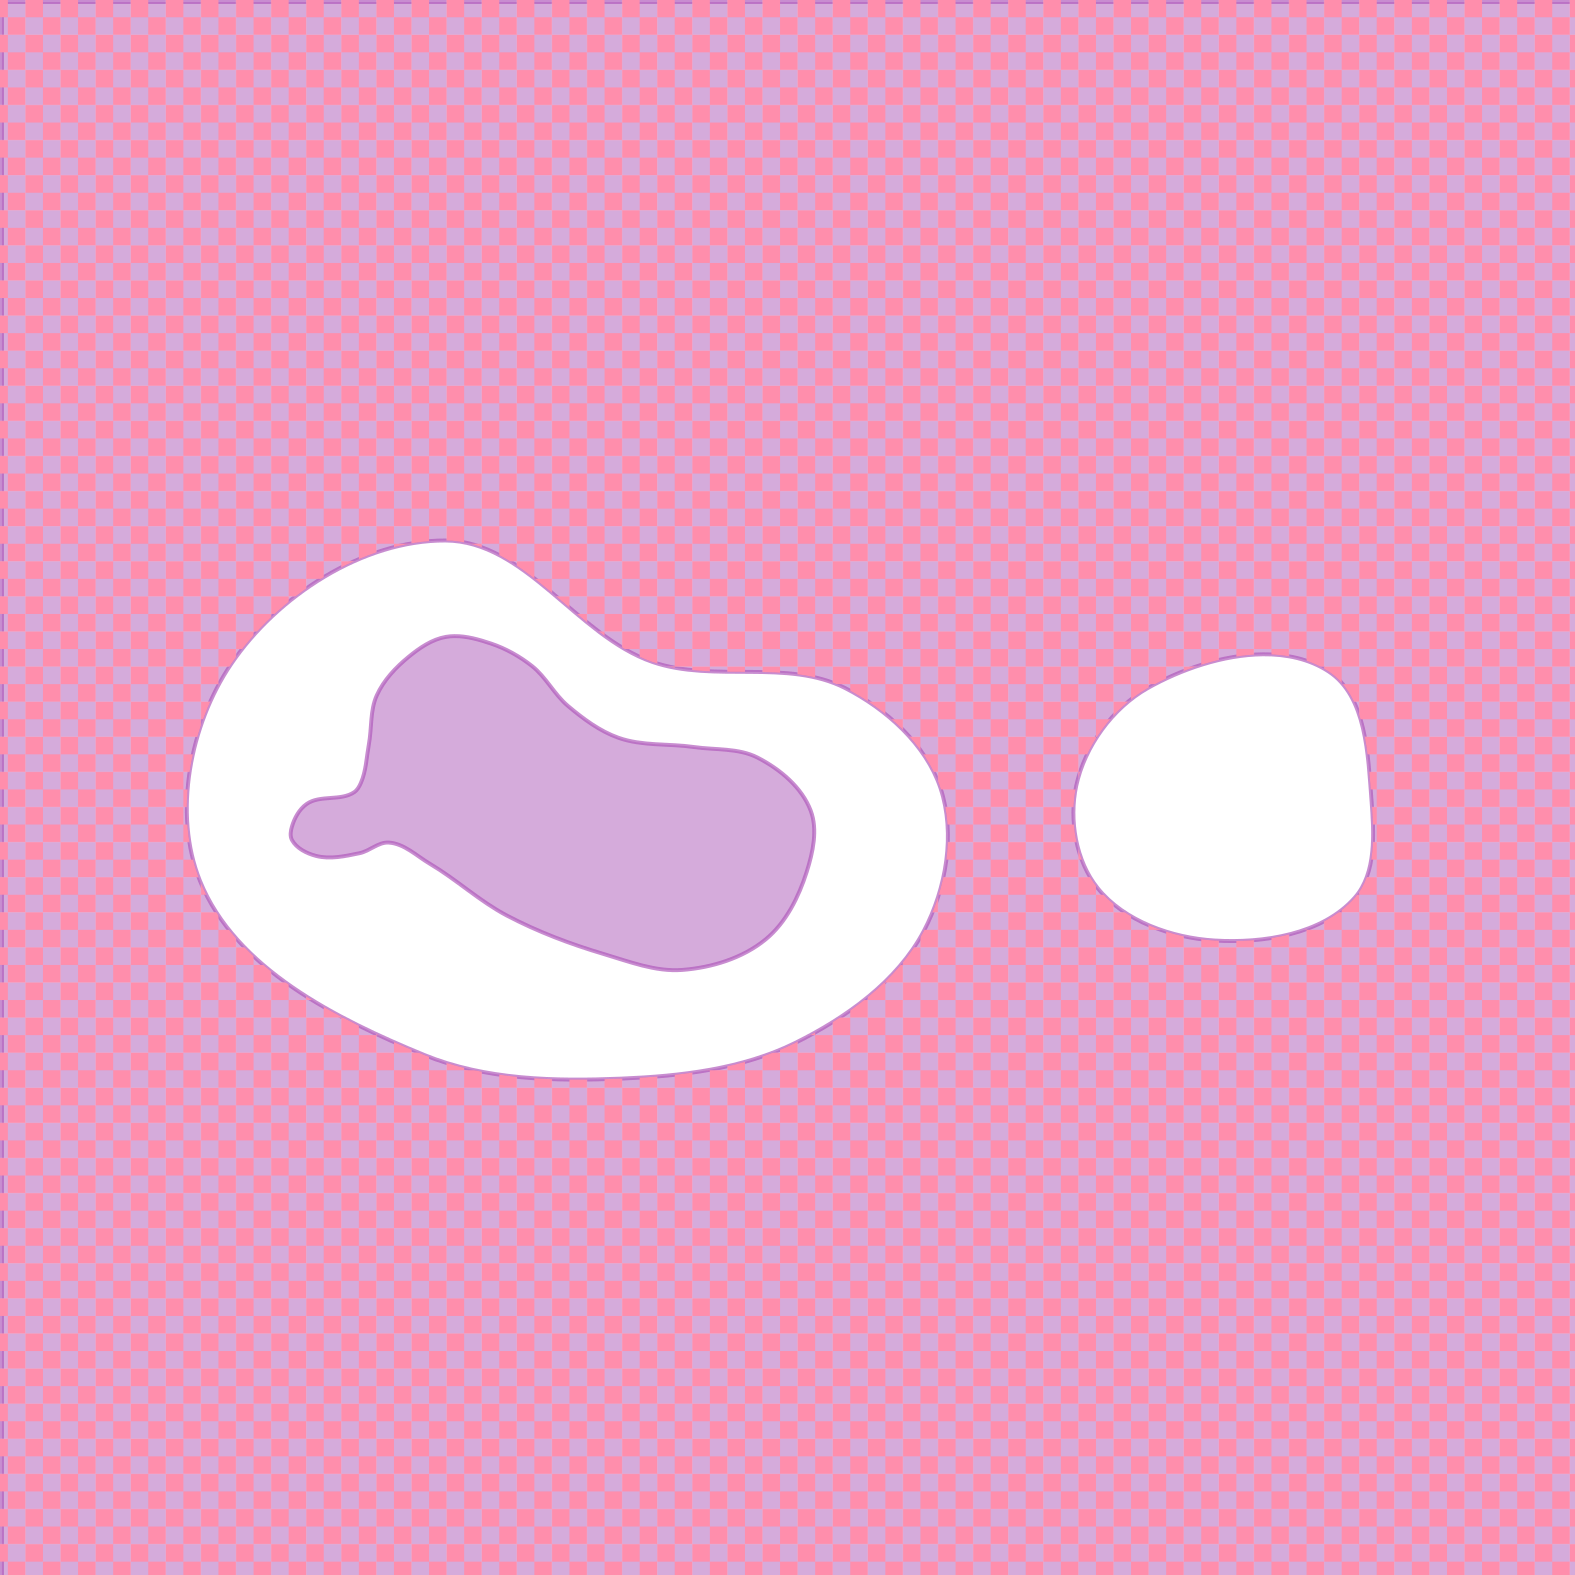
\includegraphics[trim=50 250 50 300, clip, width=0.5\textwidth]{figures/ass1_2cover/PQ2comp}%
  \end{textblock*}

  \begin{textblock*}{6cm}(6cm,4cm)
    \centering
    
\includegraphics[trim=50 250 50 300, clip, width=0.5\textwidth]{figures/ass1_2/DB1comp}%
  \end{textblock*}
  \begin{textblock*}{6cm}(6cm,6.75cm)
    \centering
    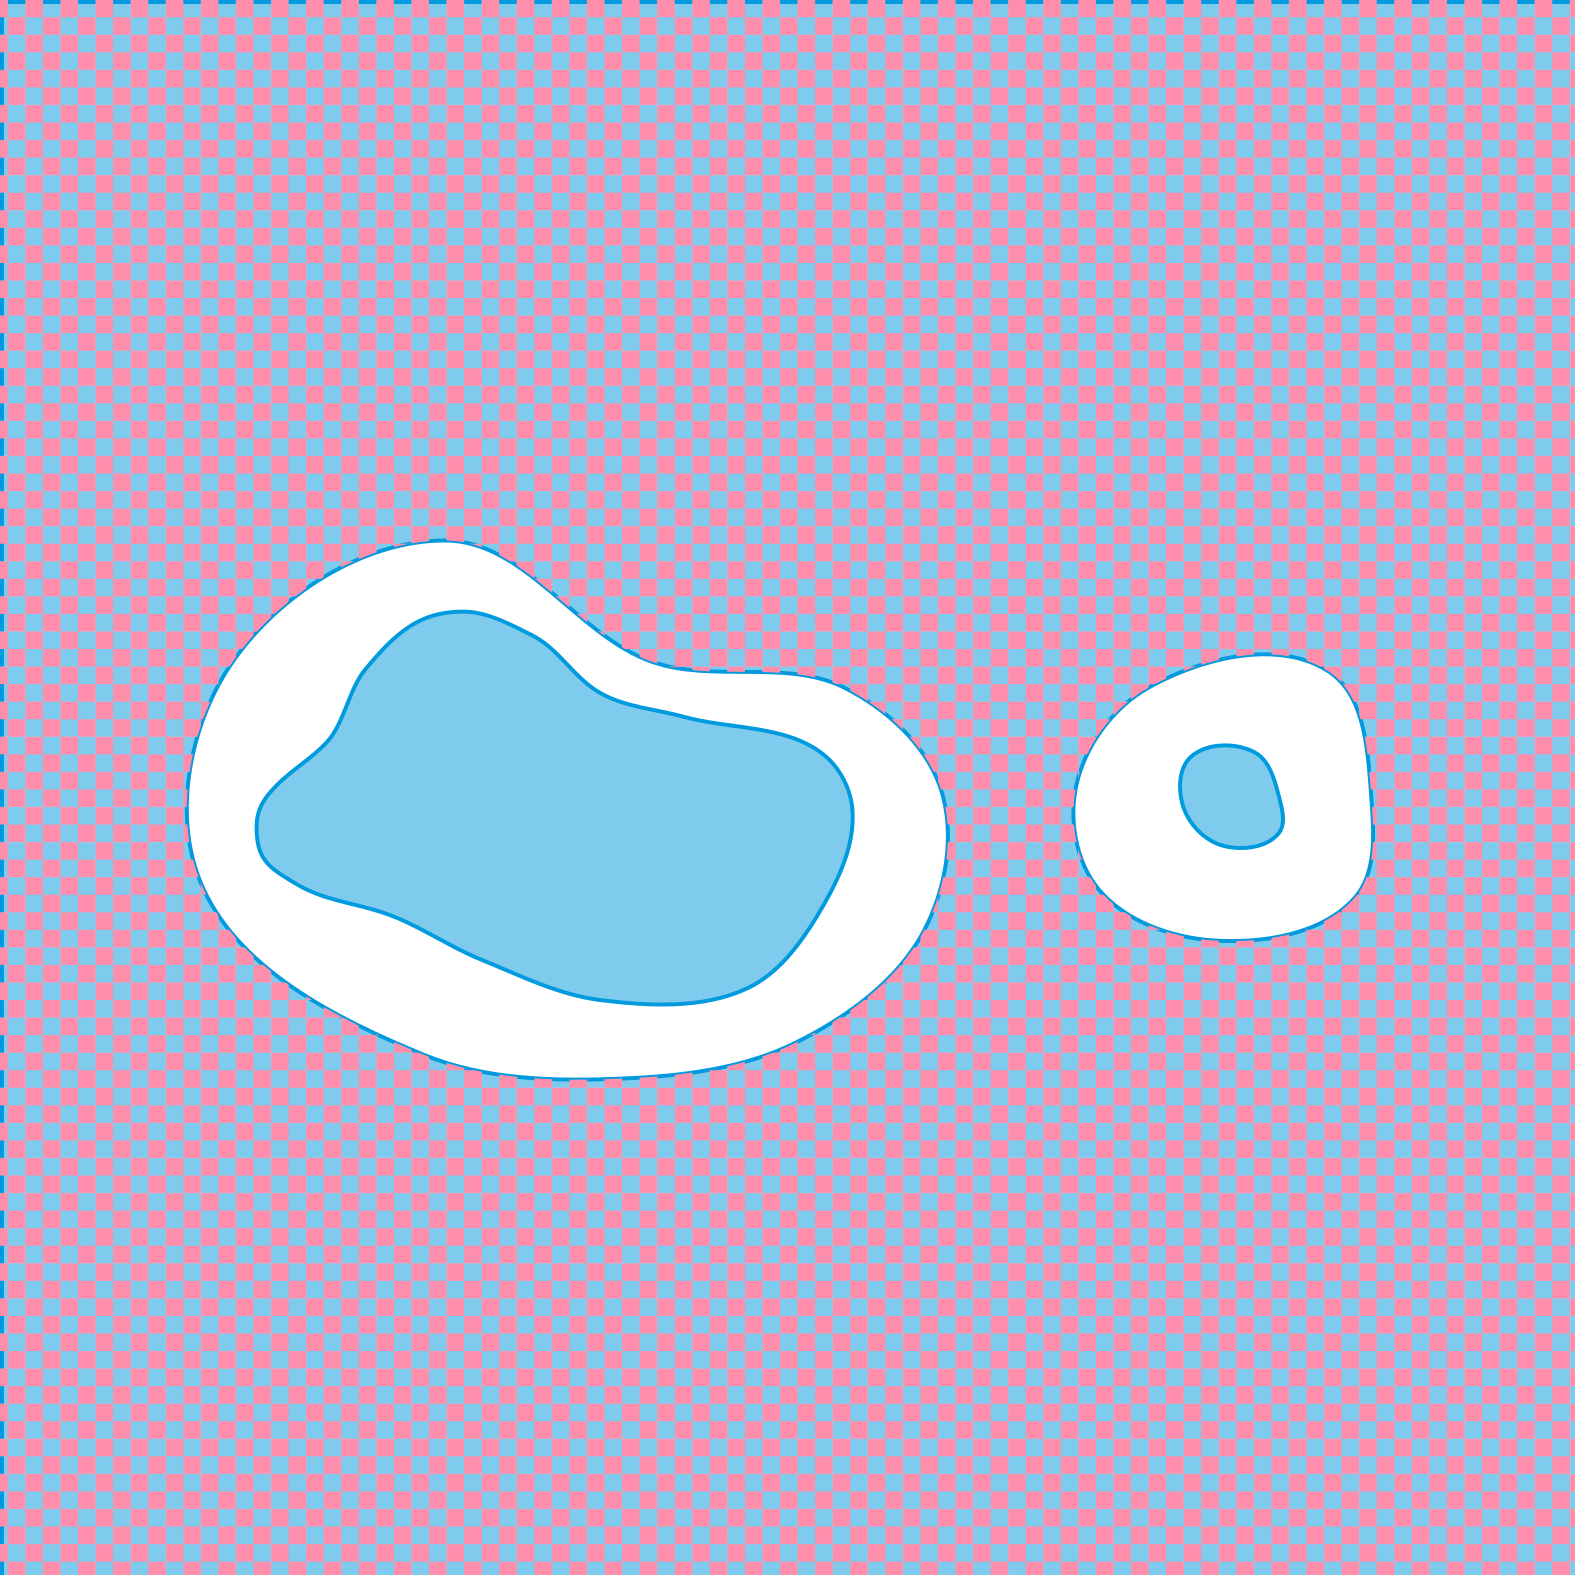
\includegraphics[trim=50 250 50 300, clip, width=0.5\textwidth]{figures/ass1_2cover/PQ1comp}%
  \end{textblock*}

  % \begin{textblock*}{11cm}(1cm,5cm)
  %   \[\begin{tikzcd}[ampersand replacement=\&]
  %     \hom_0(\overline{B_1},\overline{D})\arrow{d}{m} \arrow{r}{j} \&
  %     \hom_0(\overline{B_\omega}, \overline{D}) \arrow{d}{\ell} \\
  %     %
  %     \hom_0(\overline{Q_1^\delta}, \overline{P^\delta}) \arrow{r}{i} \&
  %     \hom_0(\overline{Q_0^\delta}, \overline{P^\delta}).
  %   \end{tikzcd}\]
  % \end{textblock*}
\end{frame}

\begin{frame}
  \begin{textblock*}{12cm}(0cm,1cm)
    \begin{small}
    \begin{description}
      \item[Goal:] Show $\ell : \hom_0(\overline{B_\omega}, \overline{D})\to \hom_0(\overline{Q^\delta},\overline{P^\delta})$ is injective.
      \item[Method:] Check
      \[\only<1-2>{ {\color<2>{red} \mathbf{rk}~\hom_0((\overline{Q_1^\delta}, \overline{P^\delta})\hookrightarrow (\overline{Q_0^\delta}, \overline{P^\delta}))}\geq \mathbf{dim}~\hom_0(D\setminus B_\omega)}
        \only<3>{\mathbf{rk}~\hom_d((P^\delta, Q_0^\delta)\hookrightarrow (P^\delta, Q_1^\delta)) \geq \mathbf{dim}~\hom_0(D\setminus B_\omega)}.\]
    \end{description}
    \end{small}
  \end{textblock*}

  \begin{textblock*}{11cm}(1cm,4cm)
    {\color{red} Duality:} $\hom_d(X, Y)\cong\hom_0(\overline{Y}, \overline{X}).$
  \end{textblock*}

  \begin{textblock*}{12cm}(0.5cm,5.5cm)
    \includegraphics<1-2>[trim=50 250 50 300, clip, width=0.4\textwidth]{figures/ass1_2cover/PQ2comp}
    \includegraphics<3>[trim=50 250 50 300, clip, width=0.4\textwidth]{figures/ass1_2cover/PQ2}\hspace{6ex}%
      \includegraphics<1-2>[trim=50 250 50 300, clip, width=0.4\textwidth]{figures/ass1_2cover/PQ1comp}
      \includegraphics<3>[trim=50 250 50 300, clip, width=0.4\textwidth]{figures/ass1_2cover/PQ1}
  \end{textblock*}
\end{frame}
